%%% -*-LaTeX-*-

\chapter{Bw-Trees}
\label{chap:bw-tree}
\section{Lock-free Indexing}

To show how these NIC features can be applied to in-memory database systems,
we now examine a data structure that is well-positioned to take advantage
of them.
The Bw-Tree~\cite{bw-tree} is an atomic record store designed for extreme
concurrency. It is an ordered index that supports basic record create, update,
and delete (CRUD) operations in addition to search and range scans.  It is
fully lock-free and non-blocking, and is optimized for modern multicore
workloads. It can store to flash, but is also intended for in-memory
workloads; it serves as the ordered secondary index structure for in-memory SQL
Server Hekaton~\cite{hekaton} engine.

In many ways, the Bw-Tree is a conventional paged B-link tree,
but it also has unique characteristics that interact with network-layer
design choices. Its lock-freedom, its elimination of update-in-place,
and its lazily consolidation of updated records in virtual memory give it
tremendous flexibility in how query results are transmitted by the NIC.

Records may be embedded within leaf pages, or the leaf pages may
only contain pointers to data records. When used as a secondary index,
typically leaf pages would contain pointers, since otherwise each record would
have to be materialized twice and the copies would need to be kept consistent.

\begin{figure}[t]
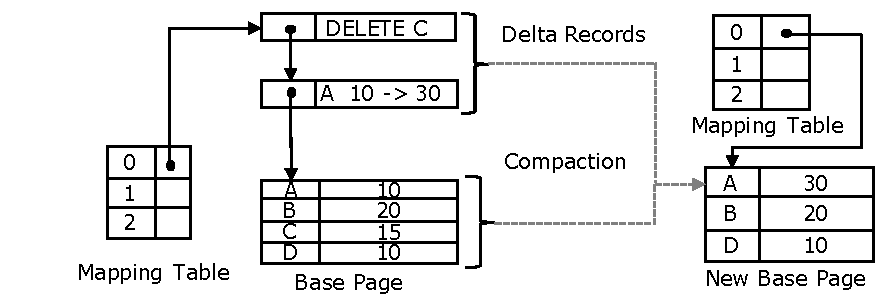
\includegraphics[width=\textwidth]{fig-bwtree.pdf}
\caption{ The structure of a Bw-Tree.}
\label{fig:bw-tree}
\end{figure}

The key challenge in a lock-free structure is providing atomic reads, updates,
inserts, and deletes without ever being able to quiesce ongoing operations (not
even on portions of the tree). Bw-Tree solves this problem by eliminating
update-in-place. All mutations are written to newly allocated memory, then
the changes are installed with a single atomic compare-and-swap instruction
that publishes the change.  Figure~\ref{fig:bw-tree} shows how this works.
In place update are avoided by creating delta records ``off to the side'' 
that describe a logical modification to a page. Delta records are
prefixed to a chain ultimately attached to a base page.  When delta chains
grow long they are compacted together with the base page to create a new base page.
All references to pages are translated through a mapping table that maps page
numbers to virtual addresses. This allows pages to be relocated in memory, and
it allows the contents of a page to swapped with a single atomic
compare-and-swap (CAS) operation.

One of the key innovations of the Bw-Tree is its use of {\em delta records},
which make updates inexpensive.
Delta records allow the Bw-Tree to logically modify the
contents of an existing page without blocking concurrent page readers, without
atomicity issues, and without recopying the entire contents of the page for
each update.  Whenever a mutation is made to a page, a small record is
allocated, and the logical operation is recorded within this delta record. The delta
record contains a pointer to the page that it logically modifies. It
is then atomically installed by performing a CAS operation on the
mapping table that re-points the virtual address for a particular page number
to the address of the delta record.

Some threads already reading the original page contents may not see
the update, but all future operations on the Bw-Tree that access that page
will see the delta record. As readers traverse the tree, they consider
the base pages to be logically augmented by their delta records. Delta records
can be chained together up to a configurable length.  When the chain becomes
too long, a new base page is formed that combines the original base page
contents with the updates from the deltas. The new page is swapped-in
the same way as other updates.

Read operations that run concurrent to update operations can observe superseded
pages and delta records, so their garbage collection must be deferred.
To solve this, each thread that
accesses the tree and each unlinked object is associated with a current {\em epoch}.
The global epoch is periodically incremented. Memory for an unlinked object can be
recycled when no thread belongs to its epoch or any earlier epoch.
The epoch mechanism gives operations consistent reads of the
tree, even while concurrent updates are ongoing. However, there is a
cost; if operations take a long time they remain active within their epoch and
prevent reclamation of memory that has been unlinked from the data structure.

\section{NIC Implications for Bw-Tree}

Lock-freedom has major implications on the in-memory layout of the
Bw-Tree. Most importantly, readers (such as the NIC DMA engine) can collect a
consistent view of the tree without interference from writers, and holding that
view consistent cannot stall concurrent readers or writers to the tree.  This
natural record stability fits with the zero-copy capabilities of modern NICs;
because the NIC's DMA engine is oblivious to any locks in the database engine,
structures requiring locking for updates would have to consider the NIC to
have a non-preemtible read lock for the entire memory region until the DMA completes.
Instead of copying records ``out'' of the data structure for transmission,
records can be accessed directly by the NIC. Eliminating the explicit copy of
the records into transmit buffers can save database server CPU and memory
bandwidth.

Page consolidation can also benefit the NIC and improve performance.  Records
in the Bw-Tree are opportunistically packed into contiguous pages in virtual
memory, but the view of a page is often augmented with (potentially many)
small delta
records that are scattered throughout memory.
A database might save CPU and memory bandwidth by more
aggressively deferring or even eliminating consolidation of records into
contiguous regions of memory or pages. We show in
our evalutation that highly discontinuous data can slow
transmission throughput but that aggressive consolidation is inefficient; delta
records can dramatically reduce consolidation overheads while keeping records
sufficiently contiguous to make the NIC more efficient.

Overall, we seek to answer these key questions:
\begin{itemize}
\item
When should records be transmitted directly from a Bw-Tree? Are there cases
where explicitly copying records into a transmit buffer is preferable to gather
DMA operations?
\item
How aggressive should a Bw-Tree be in consolidating records to benefit individual
clients and to minimize database server load?
\item
How does zero-copy impact state reclamation in the Bw-Tree? Might long transmit
times hinder performance by delaying garbage collection of stale records?
\end{itemize}

% Answering these questions?
% - When to tx zero copy versus not?
% - Show tx perf CPU use.


% K: Indexes in modern databases sustain million/op/s.

% K: To support extreme concurrency sometimes lock-free [cite BwTree, ART]

% K: Range scan performance key. But raises key question? How to inexpensively
% get the data to the NIC?

% K: Simplest approach: copy-out results and transmit. Tradtionally this would
% have yielded three copies. One into the results buffer, one for the kernel to
% copy the results into packet buffers, and one for the NIC to DMA the data for
% transmit.

% What about zero-copy? Several problems:
%  - atomicity
%  - garbage collection and object lifetime
%  - packaging the objects for efficient transmit.
%    - pre-package? (paged structures)
%    - use NIC DMA engine?
% Key question? What are the gains?
%  - Reduced copies -> reduced memory bandwidth use, reduced CPU time

% K: Zero-copy? Then data structure must be tied into messaging layer. Can work
% with epoch-based GC, but what about long scans? Could hold back GC and stall
% tree in the limit.
